\documentclass[a4paper]{article}
\usepackage{graphicx}
\usepackage{amsmath}
\usepackage{float}
\usepackage{geometry}
\usepackage{listings}
\usepackage{multicol}
\usepackage{float}
\usepackage{caption}
\usepackage{enumitem}
\usepackage[americanvoltages,fulldiodes,siunitx]{circuitikz}
\usepackage{wrapfig}
\usepackage{mathrsfs} % https://www.ctan.org/pkg/mathrsfs
\newcounter{MyCounter}
\usepackage{enumitem}
\usepackage{pgfplots}
\usepackage{subfig}	% ploting figures beside each other
\pgfplotsset{compat=1.12}

 \geometry{
 a4paper,
 total={170mm,257mm},
 left=20mm,
 top=20mm,
 }
\usepackage{fancyhdr}
\pagestyle{fancy}
\cfoot{(\space \space \space \space \textbf{\thepage}  \space \space \space)}
\renewcommand{\headrulewidth}{1pt}
\renewcommand{\footrulewidth}{1pt}
\usepackage{listings}
\usepackage{color} %red, green, blue, yellow, cyan, magenta, black, white
\definecolor{mygreen}{RGB}{28,172,0} % color values Red, Green, Blue
\definecolor{mylilas}{RGB}{170,55,241}


\begin{document}
	\lstset{language=Matlab,%
		%basicstyle=\color{red},
		breaklines=true,%
		morekeywords={matlab2tikz},
		keywordstyle=\color{blue},%
		morekeywords=[2]{1}, keywordstyle=[2]{\color{black}},
		identifierstyle=\color{black},%
		stringstyle=\color{mylilas},
		commentstyle=\color{mygreen},%
		showstringspaces=false,%without this there will be a symbol in the places where there is a space
		numbers=left,%
		numberstyle={\tiny \color{black}},% size of the numbers
		numbersep=9pt, % this defines how far the numbers are from the text
		emph=[1]{for,end,break},emphstyle=[1]\color{blue}, %some words to emphasise
		%emph=[2]{word1,word2}, emphstyle=[2]{style},    
	}
	





	\begin{center}
	\textbf{
	\\In the name of God
		}\\
	
	\vspace{2cm}
	
\includegraphics[scale=.35]{logo1.png}\\
	\vspace{0.5cm}
	\begin{Large}
	\textbf{
	\\Sharif University of Technology
	\vspace{0.5cm}
	\\School of Electrical Engineering
	}
	\end{Large}
	\vspace{2cm}
	\begin{huge}
	\textbf{
	\\Convex Optimization
	\vspace{0.75cm}
‍
	\\Homework Nr. 1
	}
	\end{huge}
	\vspace{2cm}
	\begin{Large}
	\textbf{
	\\Dr. Babazadeh
	\vspace{2cm}
	\\Taha Entesari
	\vspace{0.75cm}
	\\95101117
	}
	\end{Large}
	
\end{center}

\thispagestyle{empty}
\newpage
\subsection*{Problem 6}
\begin{Large}
	Below the simulation results for different values of \textbf{n} are presented. As it can clearly be seen from the figures, the set is \textit{convex}. These pictures are just sample results and if $ Q_1 $ and $ Q_2 $ change, we will get different results but the set still remains convex for all symmetric $ Q $.
	\begin{figure}[!h]
		\begin{center}
			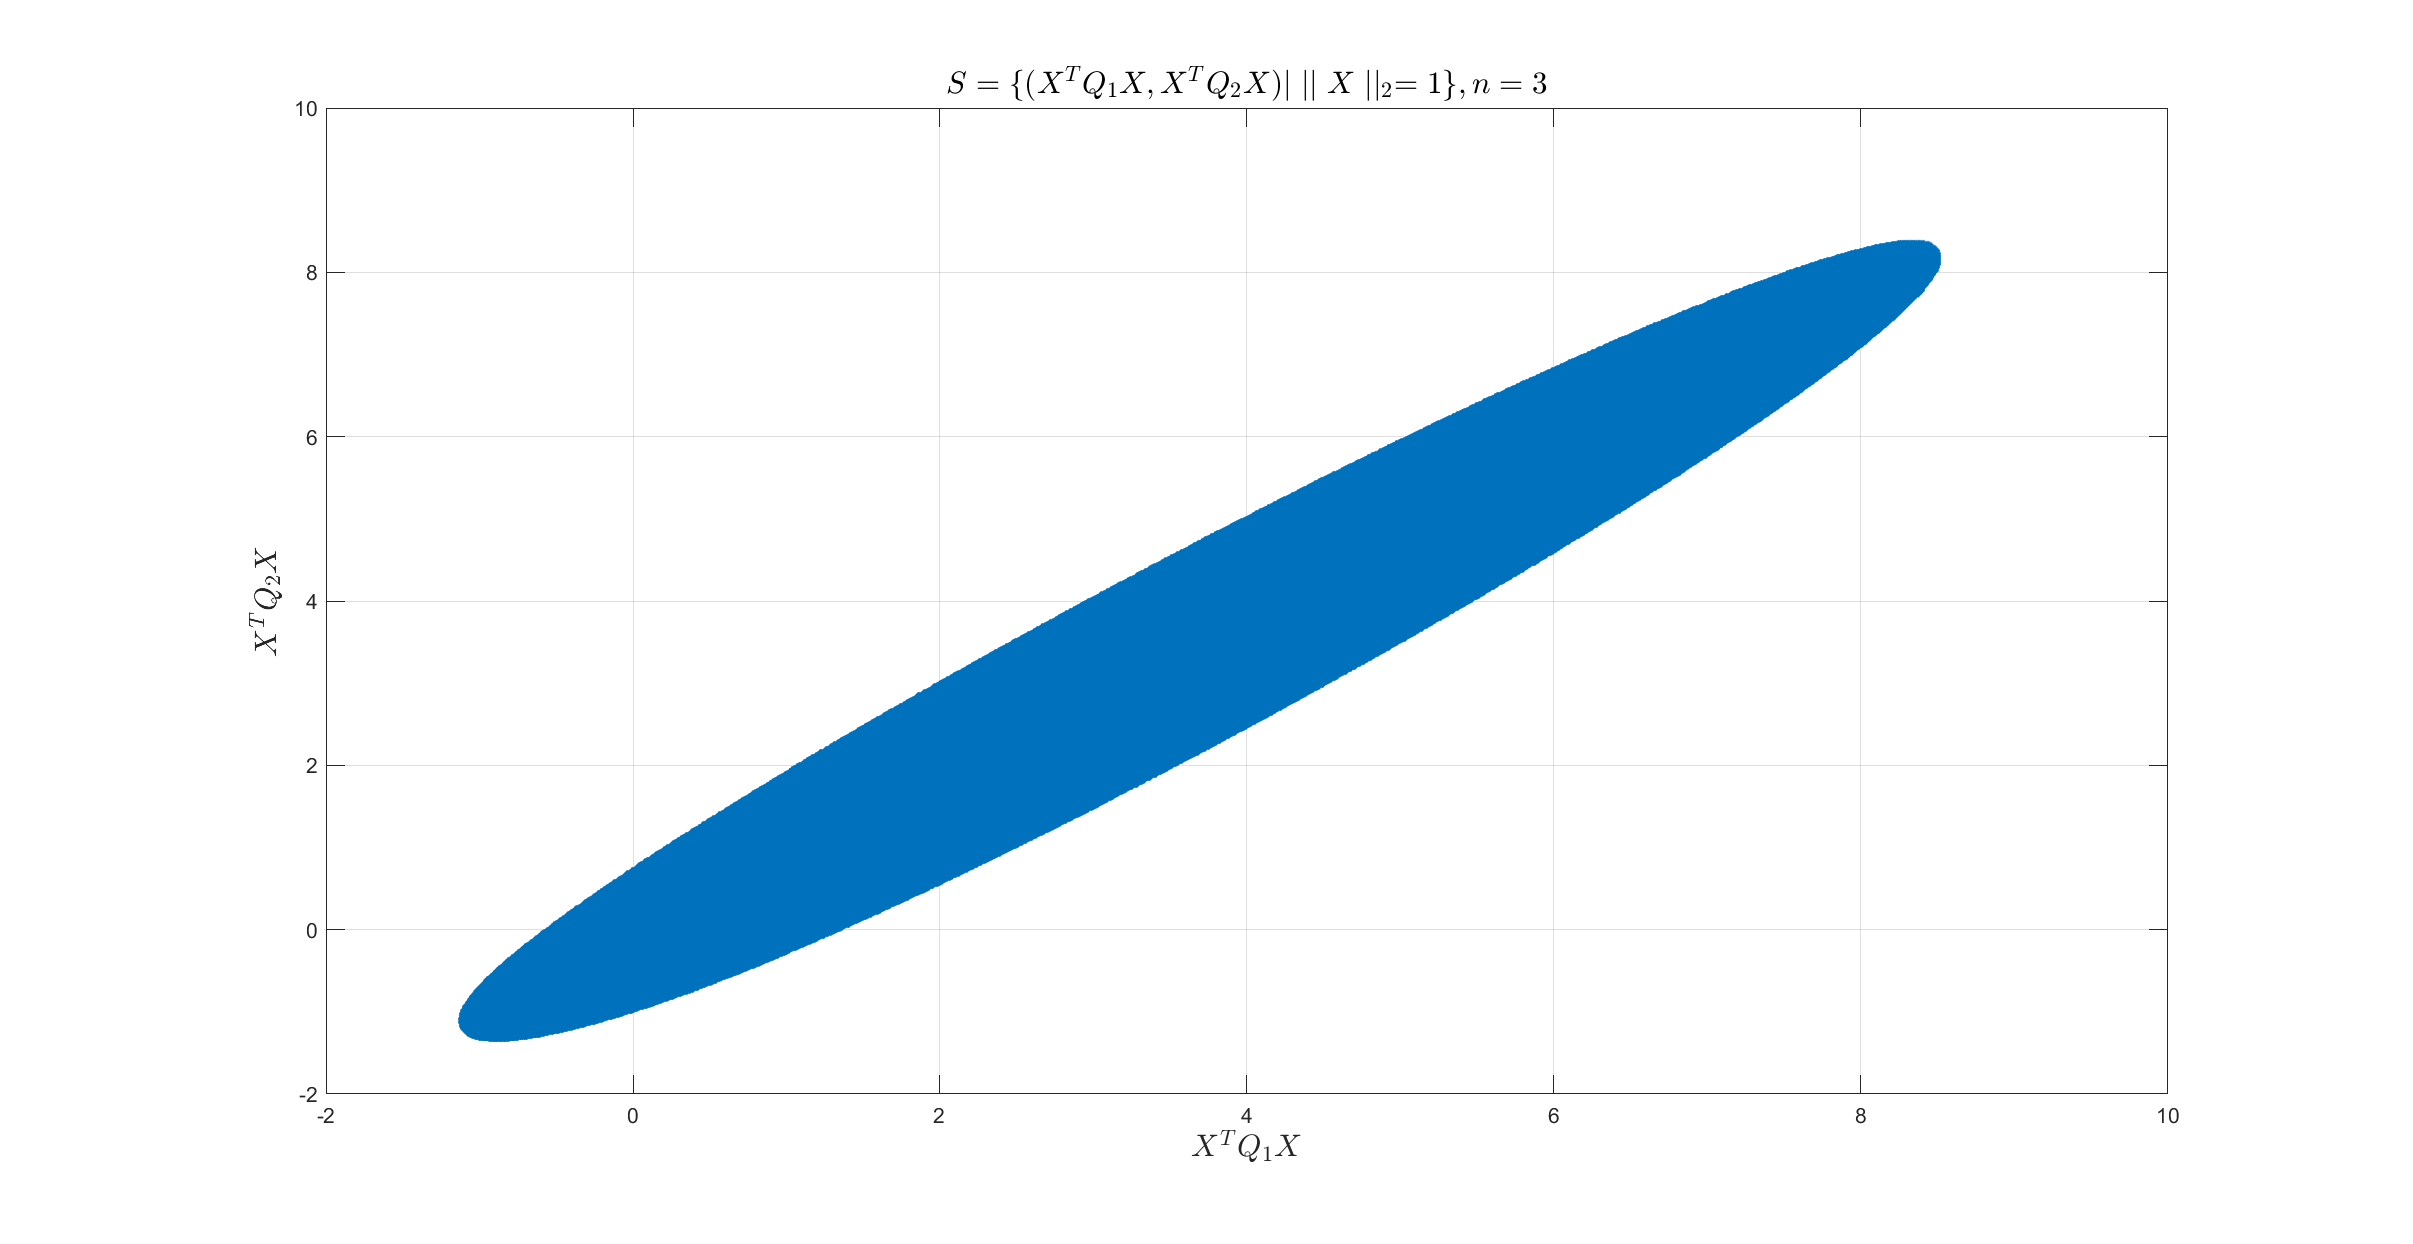
\includegraphics[scale=.45]{q13}
		\end{center}
	\end{figure}
	\begin{figure}[!h]
		\begin{center}
			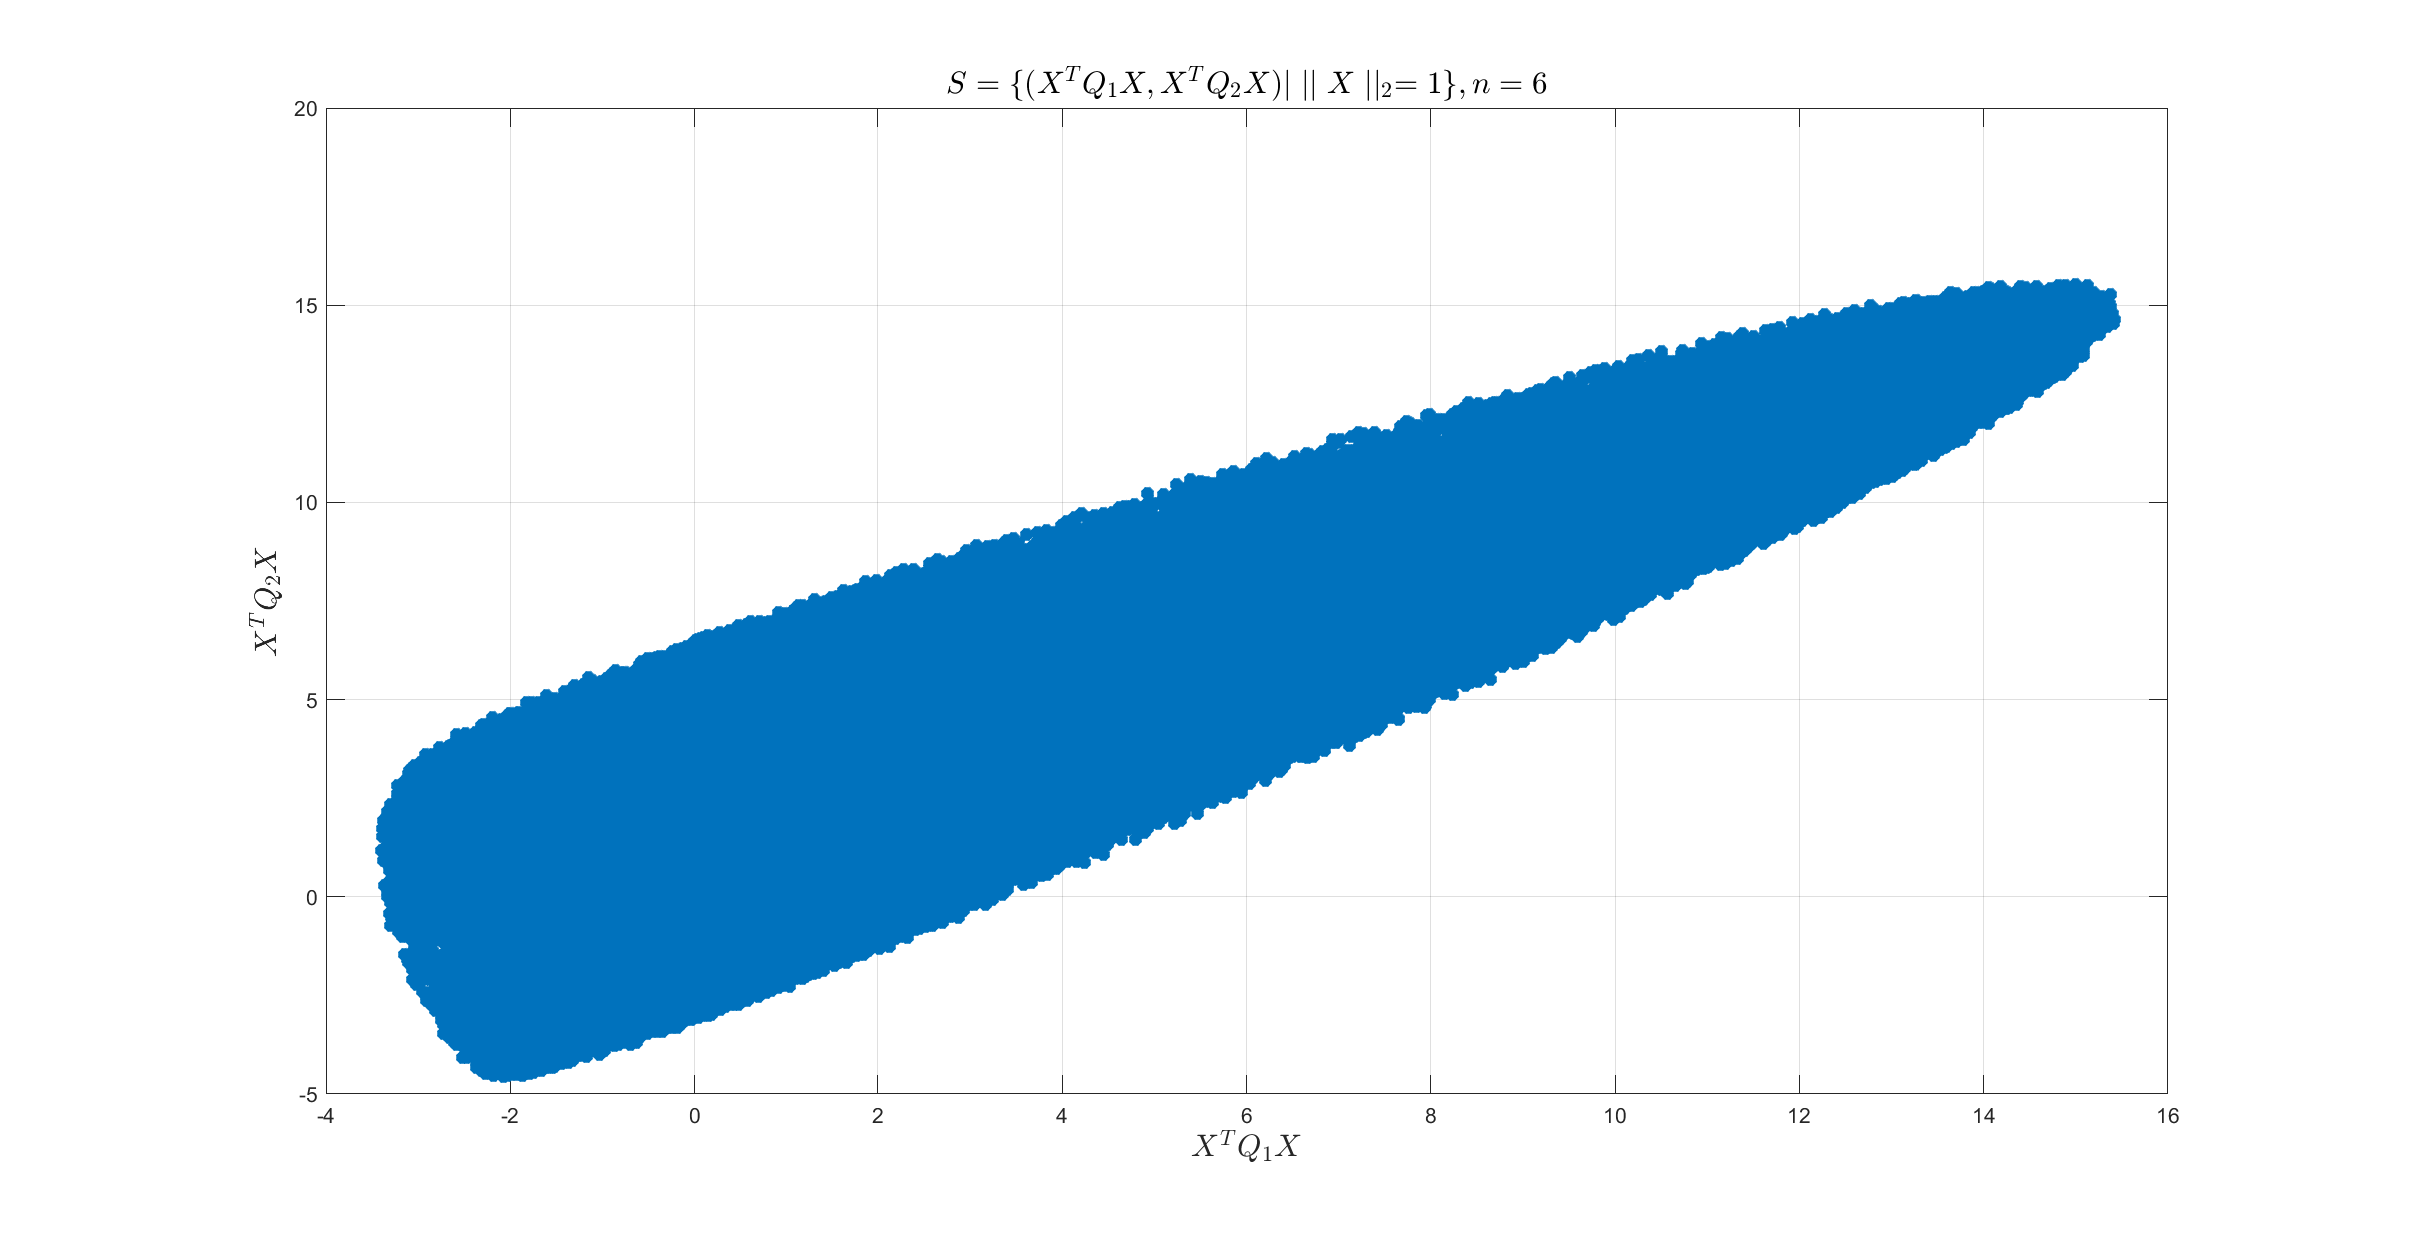
\includegraphics[scale=.45]{q16}
		\end{center}
	\end{figure}
	\begin{figure}[!h]
		\begin{center}
			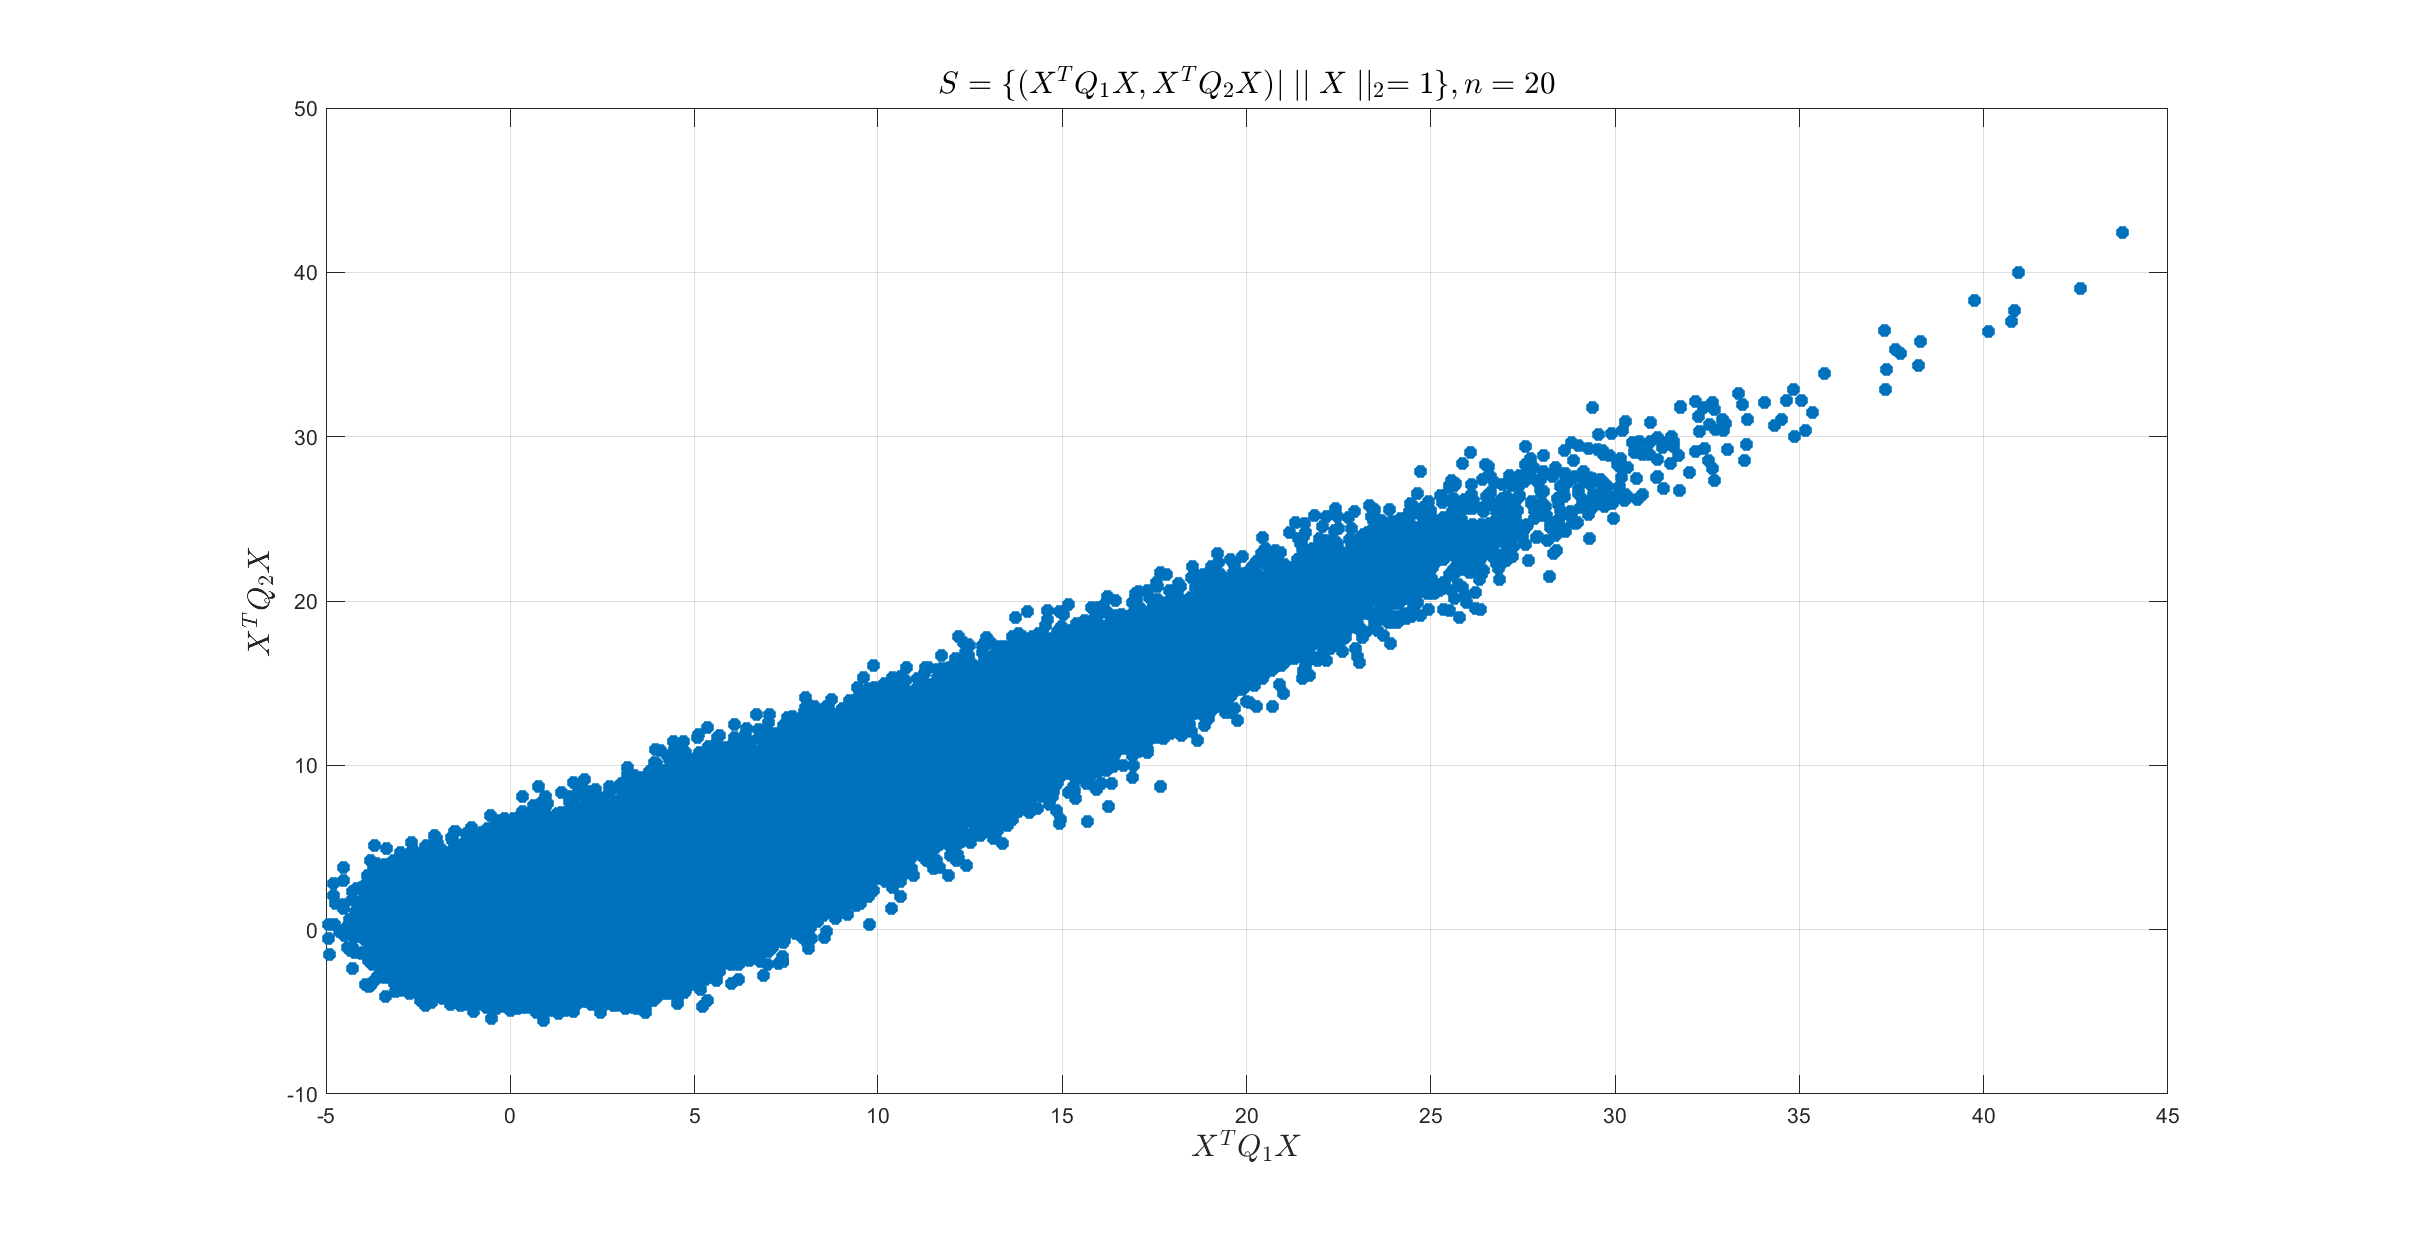
\includegraphics[scale=.45]{q120}
		\end{center}
	\end{figure}
\newpage
	As it is mentioned in the question, the matrices $ Q_1 $ and $ Q_2 $ need to have $ n>2 $. For n=2, the set defined by the points is the boundary of a convex set. A sample figure is shown below:
		\begin{figure}[!h]
		\begin{center}
			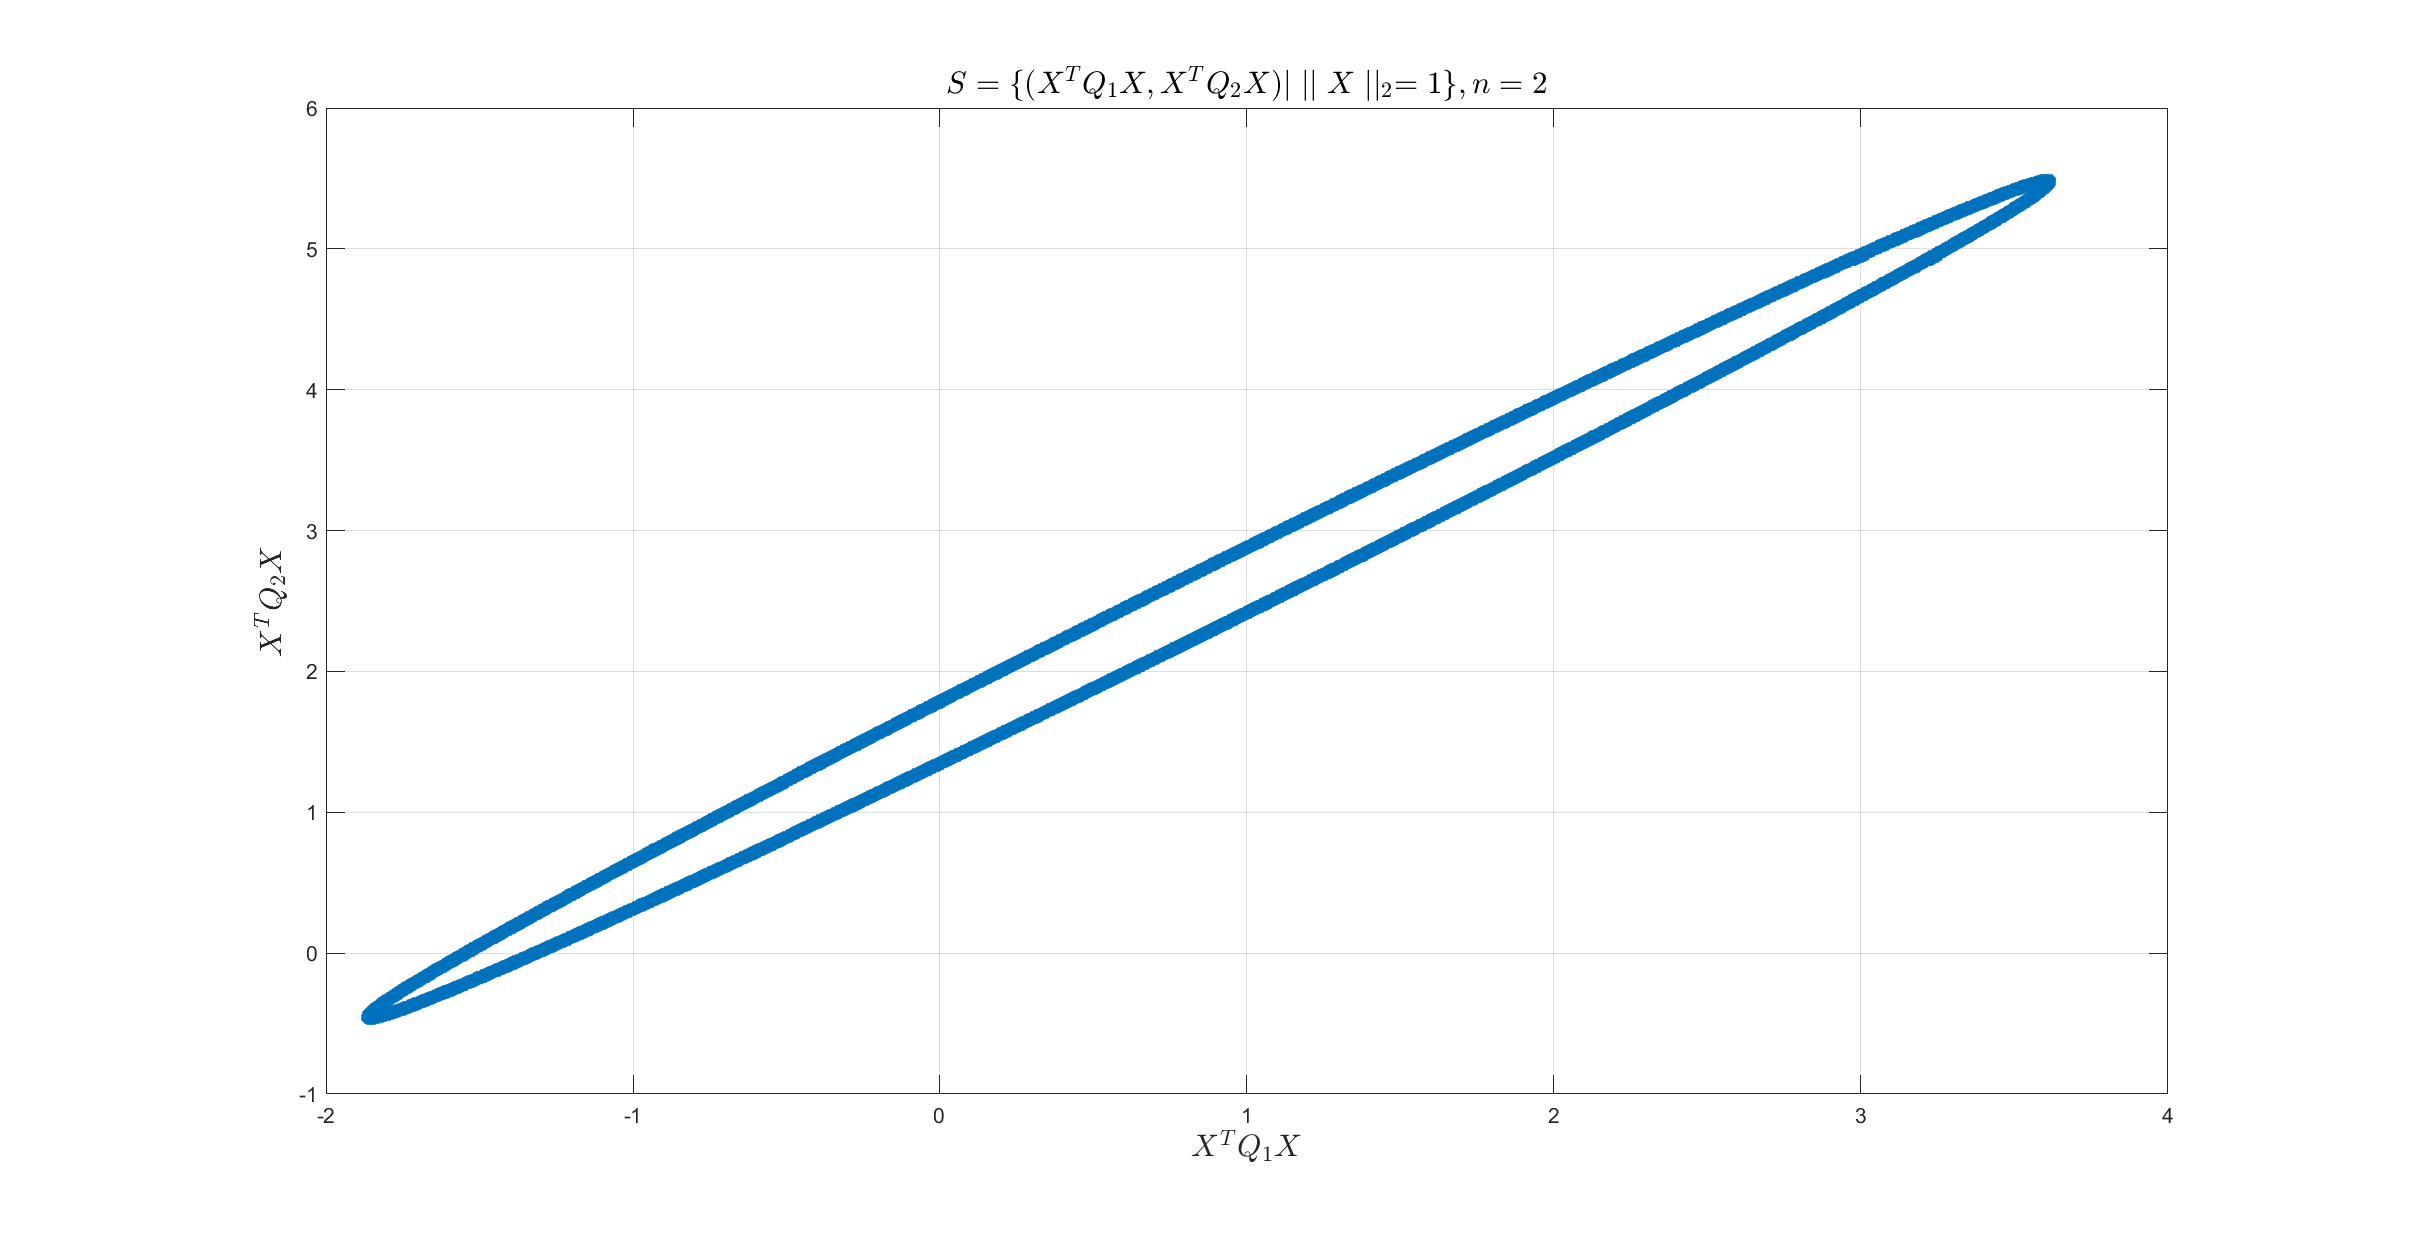
\includegraphics[scale=.45]{q12}
		\end{center}
	\end{figure}


	\newpage


	\subsection*{Problem7}
		\textbf{Part a}\\
		For this problem, first 4 vectors are randomly generated. These vectors are $ y_1, y_2, x_1, x_2 $. Each vector has elements in each quarter of $ R^2 $ plane. Using a for loop the required condition is checked and the plot is sketched using only the points that satisfy the inequality for all the generated $ x $ points. The below figure is the result and as it can be seen, the set is convex.
	\begin{figure}[!h]
		\begin{center}
			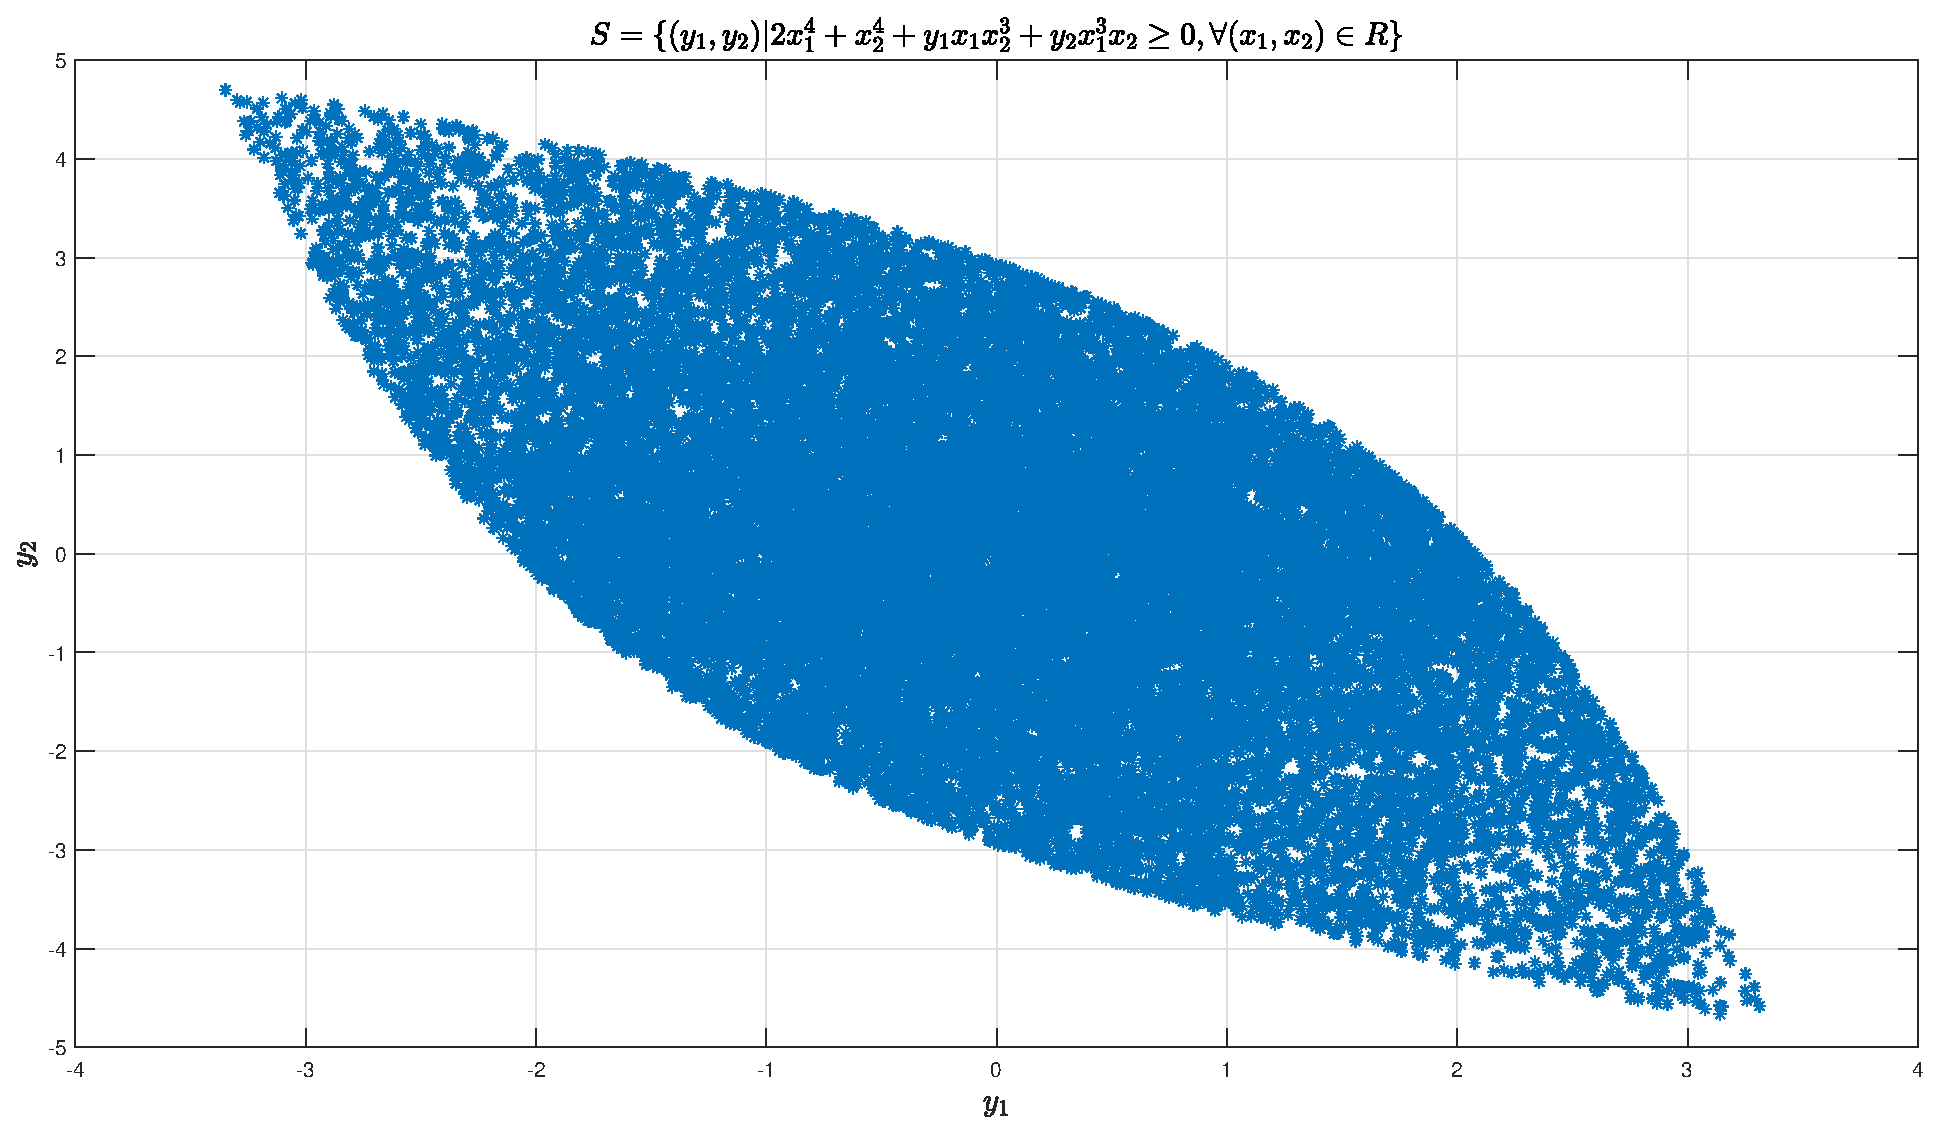
\includegraphics[scale=.45]{q7}
		\end{center}
	\end{figure}
\\\textbf{Part b}\\
Consider the given equation for a constant vector $ (x_1, x_2) $, the equation is writable as $ A^Ty+b\geq 0 $ and is thus the set of the intersection of hyperplanes and thus is convex.
	
	\newpage
	\subsection*{Problem 8}
	\textbf{Part b}\\
	Below are a few results for different k. The first image is for k=1.
	\begin{figure}[!h]
		\begin{center}
			
\includegraphics[scale=.45]{ReconstructedHajik=1}
		\end{center}
	\end{figure}
The second image is .for k=6.
	\begin{figure}[!h]
	\begin{center}
		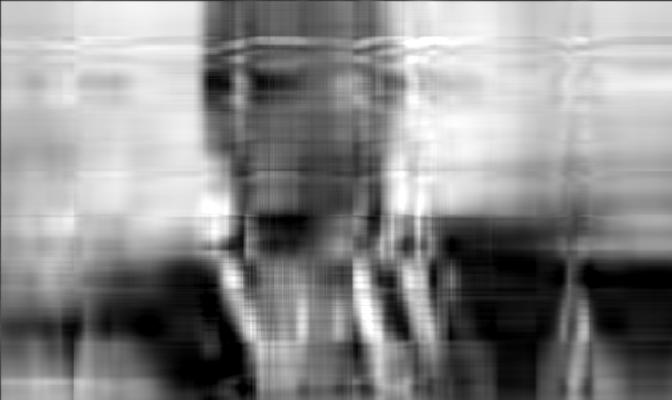
\includegraphics[scale=.45]{ReconstructedHajik=6}
	\end{center}
\end{figure}
The third image is for k=21.
	\begin{figure}[!h]
	\begin{center}
		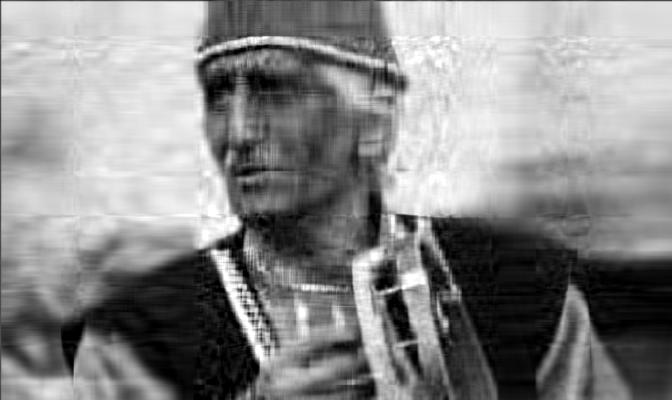
\includegraphics[scale=.45]{ReconstructedHajik=21}
	\end{center}
\end{figure}
The forth image is for k=50.
	\begin{figure}[!h]
	\begin{center}
		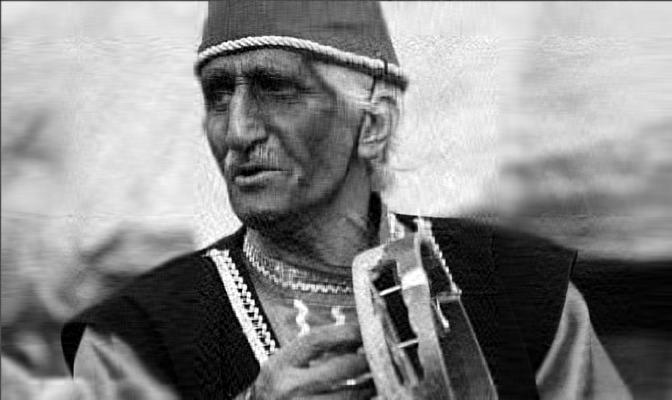
\includegraphics[scale=.45]{ReconstructedHajik=50}
	\end{center}
\end{figure}
The final image is for k=200.
\begin{figure}[!h]
	\begin{center}
		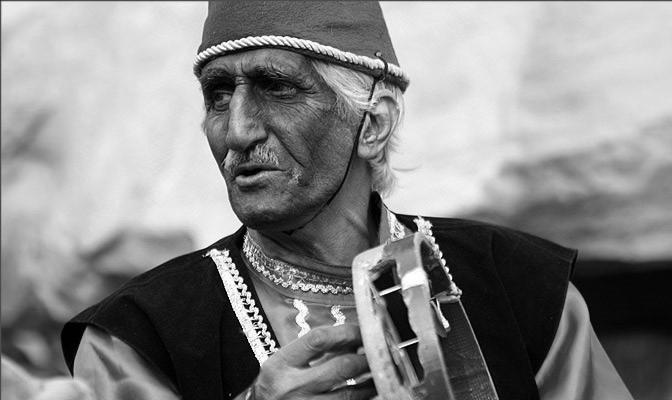
\includegraphics[scale=.45]{ReconstructedHajik=200}
	\end{center}
\end{figure}
It is evident that we can reconstruct the original signal using the k singular values and the error drops pretty quickly. For example, the following errors were recorded using MATLAB. 
\begin{figure}[!h]
	\begin{center}
		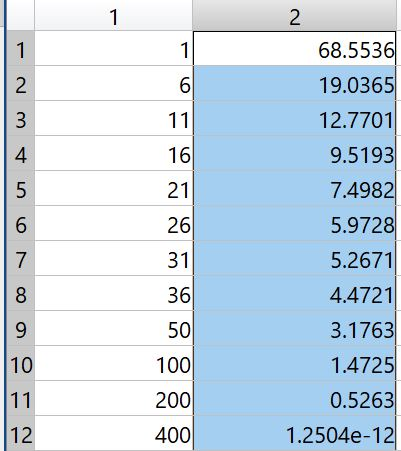
\includegraphics[scale=.45]{err}
	\end{center}
\end{figure}
The 1st column of this country is the value of k and the data on the 2nd column is the corresponding error.\\
Though it is probably not a part of the course, it is important to notice that though we have used a few number of singular values to \textit{compress} the image, this does not mean that the resultant \textit{.jpg} image will also take up less space. This is due to the encoding of the \textit{jpg} format. Quite the opposite was seen, i.e. through using 50 singular values, we get a file that takes up more space that the original black and white image. This can somewhat be understood. By using the singular value decomposition, it is possible that for example the background of the image becomes more detailed as in having less of an equal shape. Due to the nature of the \textit{jpg} encoding format, this can result in a larger file.
	\\\textbf{Part c}\\
	Looking at the final figure for the error rate, k=50 would seem like a reasonable choice since the image has most of the detail as the original image and the error is also small.
	
	
\end{Large}
\newpage
\section*{Code Appendix}
\lstinputlisting{hw1Stu95101117.m}
\end{document}

